\section{Технический проект}
\subsection{Общая характеристика организации решения задачи}

Необходимо спроектировать и разработать приложение, который должен способствовать популяризации ролевых игр.

Приложение представляет собой набор взаимосвязанных различных окон, которые сгруппированы по разделам, содержащие текстовую, графическую информацию. Приложение располагается на компьютере.

\subsection{Обоснование выбора технологии проектирования}

На сегодняшний день информационный рынок, поставляющий программные решения в выбранной сфере, предлагает множество продуктов, позволяющих достигнуть поставленной цели – разработки приложения.

\subsubsection{Описание используемых технологий и языков программирования}

В процессе разработки приложения используются программные средства и языки программирования. Каждое программное средство и каждый язык программирования применяется для круга задач, при решении которых они необходимы.

\subsubsection{Язык программирования Python}

Python –  высокоуровневый язык программирования общего назначения с динамической строгой типизацией и автоматическим управлением памятью, ориентированный на повышение производительности разработчика, читаемости кода и его качества, а также на обеспечение переносимости написанных на нём программ. Язык является полностью объектно-ориентированным в том плане, что всё является объектами. Необычной особенностью языка является выделение блоков кода отступами. Синтаксис ядра языка минималистичен, за счёт чего на практике редко возникает необходимость обращаться к документации. Сам же язык известен как интерпретируемый и используется в том числе для написания скриптов. Недостатками языка являются зачастую более низкая скорость работы и более высокое потребление памяти написанных на нём программ по сравнению с аналогичным кодом, написанным на компилируемых языках, таких как C или C++.

\subsubsection{Использование библиотеки Tkinter и реализация таймеров на Python}
	
\paragraph{Введение}
Библиотека Tkinter - это стандартная библиотека Python для создания графического пользовательского интерфейса (GUI). Она обладает широкими возможностями для создания разнообразных приложений с использованием различных виджетов, таких как кнопки, поля ввода, метки и многое другое.
	
\paragraph{Возможности Tkinter}
Вот некоторые из основных возможностей, предоставляемых библиотекой Tkinter:
	
\begin{itemize}
	\item Создание различных виджетов: кнопки, метки, поля ввода, списки и многое другое.
	\item Управление компоновкой виджетов с использованием менеджеров компоновки (например, grid, pack, place).
	\item Обработка событий, таких как щелчок мыши, нажатие клавиш и другие.
	\item Возможность создания различных диалоговых окон, таких как окна предупреждений, информационные окна и окна запроса.
	\item Поддержка многопоточности для обновления интерфейса из различных потоков выполнения.
\end{itemize}
	
\paragraph{Заключение}
Библиотека Tkinter предоставляет мощные инструменты для создания графических пользовательских интерфейсов на языке Python. Реализация таймеров на Python может быть достигнута с помощью модулей \texttt{time} или \texttt{threading}, в зависимости от конкретных требований приложения.

\subsection{Архитектура платформы для создания ролевых игр}
\subsubsection{Диаграмма компонентов классов}
Диаграмма компонентов описывает особенности физического представления разрабатываемой системы. Она позволяет определить архитектуру системы, установив зависимости между программными компонентами, в роли которых может выступать как исходный, так и исполняемый код. Основными графическими элементами диаграммы компонентов являются компоненты, интерфейсы, а также зависимости между ними. На рисунке \ref{diagram.eps:image} изображена диаграмма компонентов для проектируемой системы. Она включает в себя основной класс платформы игры Game и производные от него классы, класс Object с наследниками и их параметрами (полями и методами).
\begin{figure}[ht]
	\center{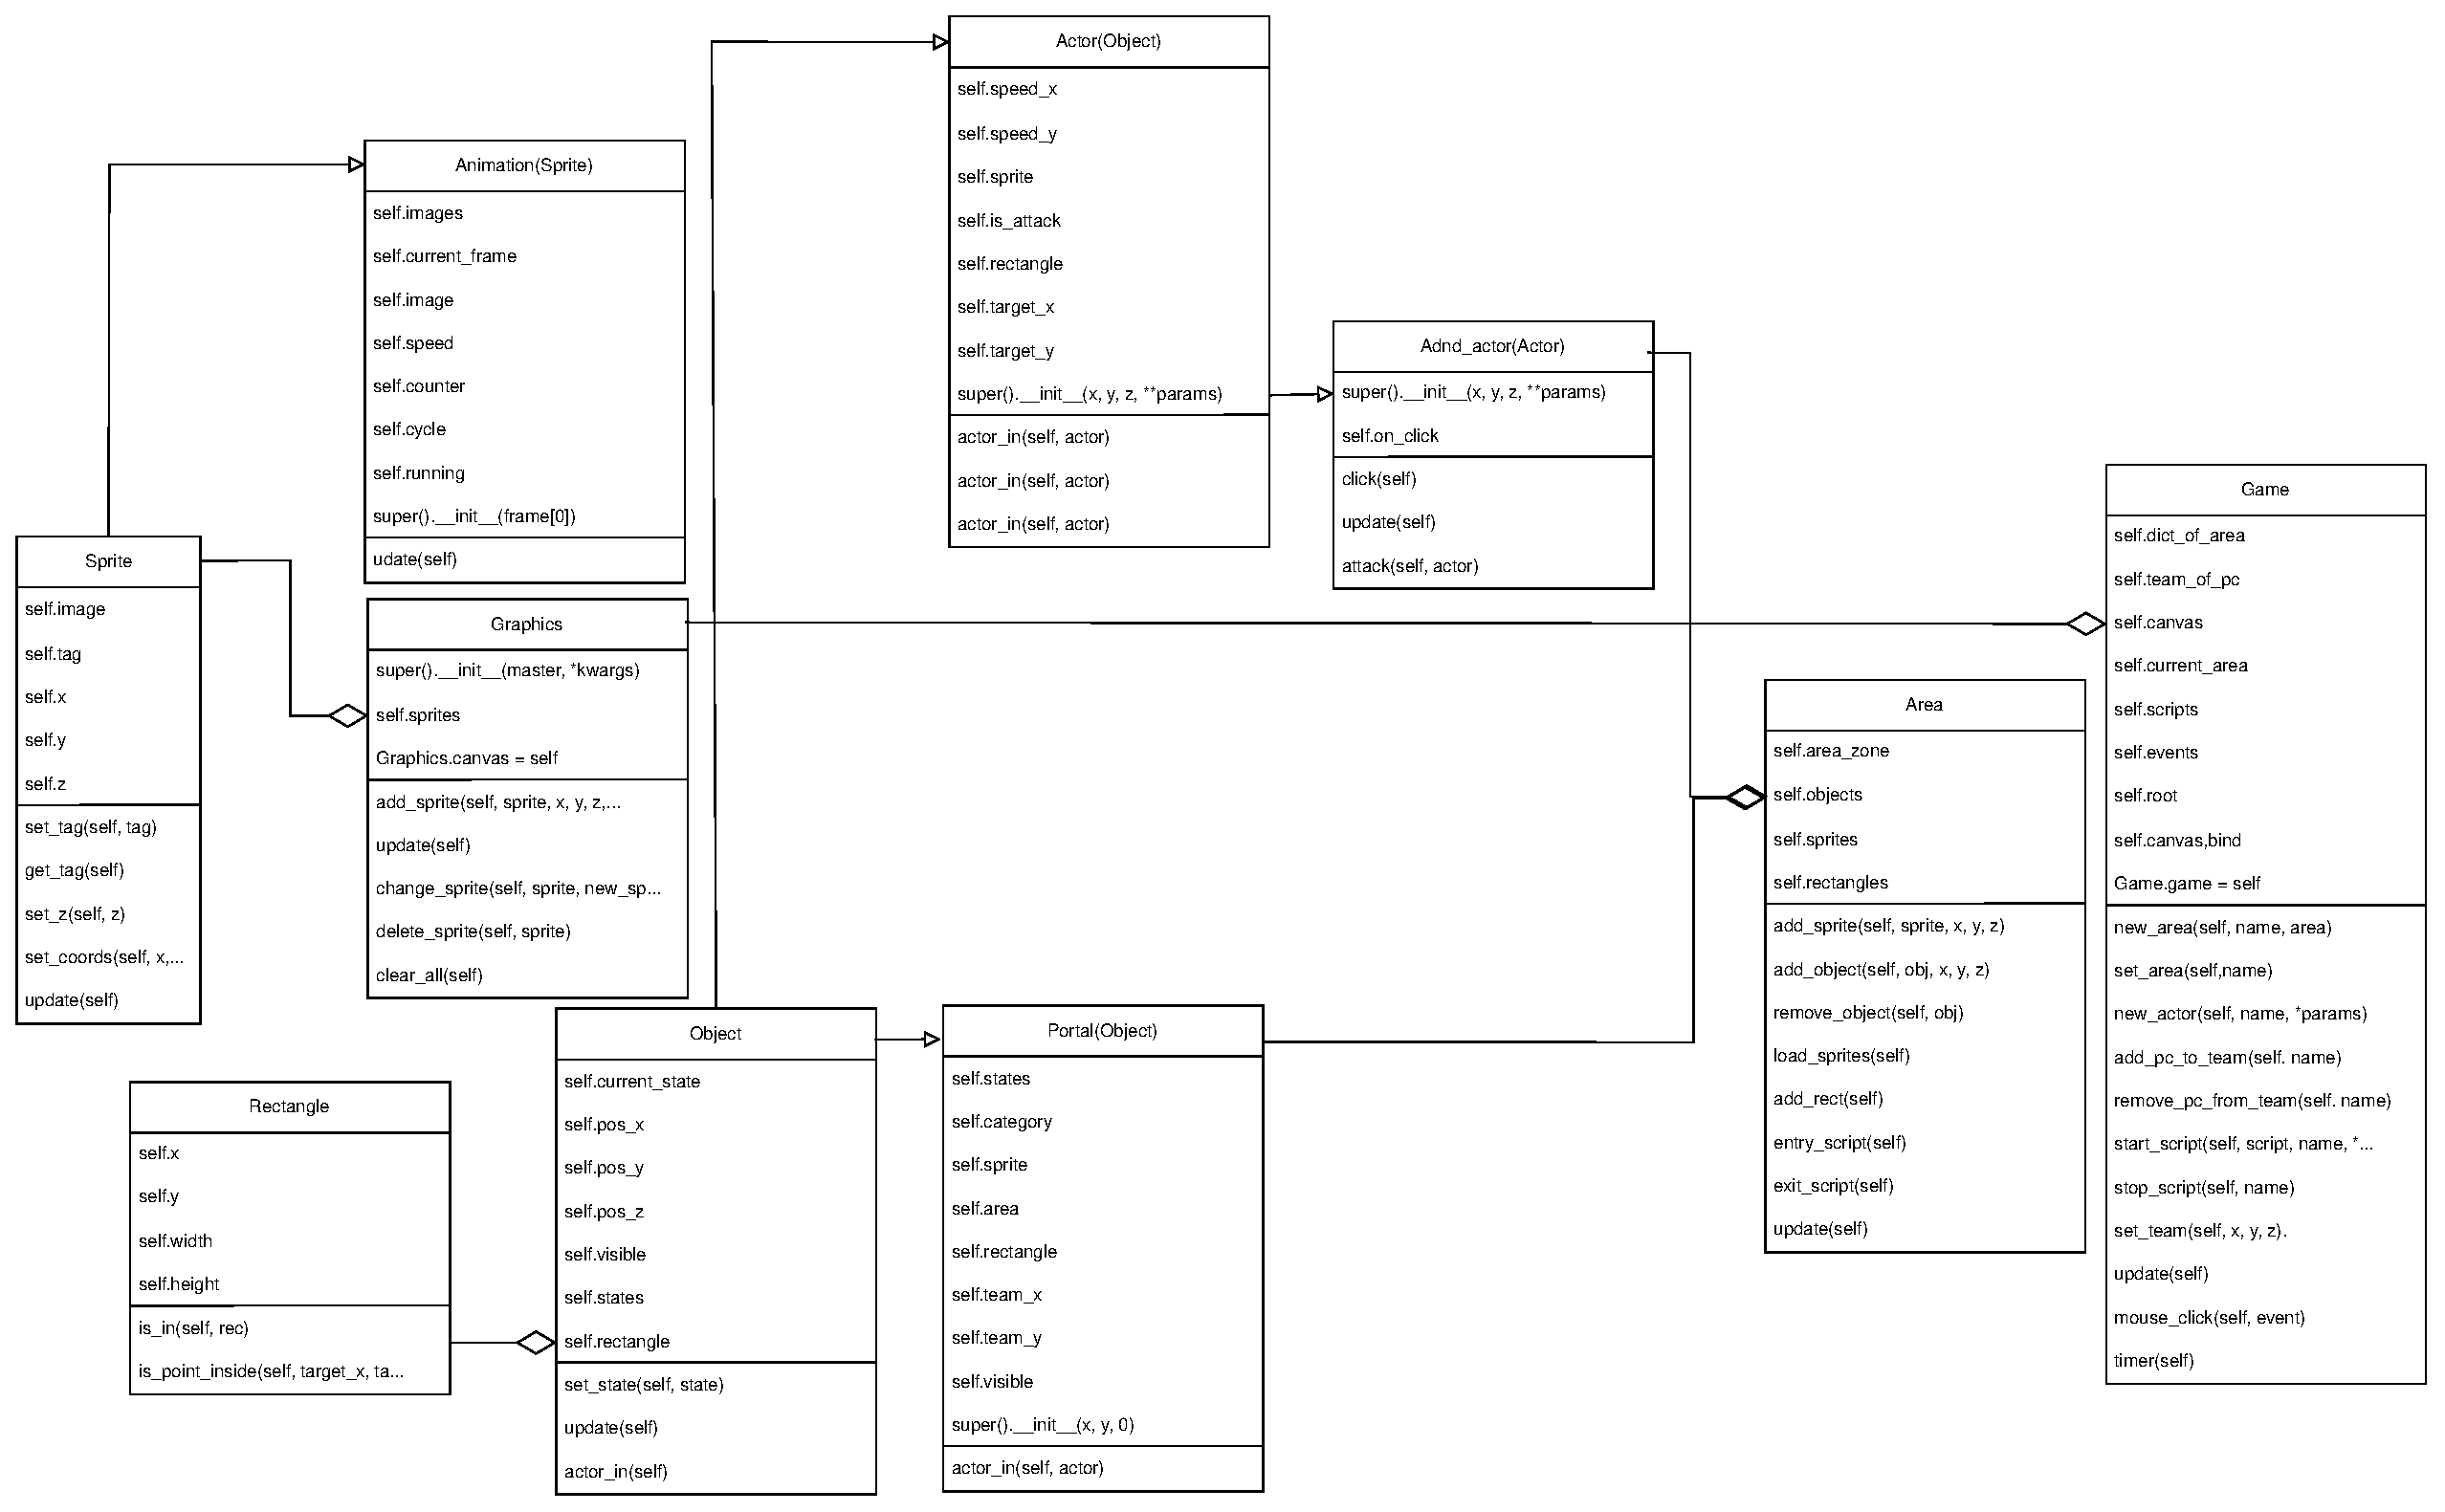
\includegraphics[width=1\linewidth]{diagram}}
	\caption{Диаграмма компонентов}
	\label{diagram:image}
\end{figure}
\paragraph{Описание классов}
\begin{enumerate}
	\item[Graphics] - класс, управляющий спрайтами. Содержит в себе:
	\begin{itemize}
		\item self.sprites - список спрайтов;
		\item add\_sprite(self, sprite x, y, z, image) - добавляет в список спрайт, сохраняет координаты;
		\item change\_sprite(self, sprite new\_sprite) - меняет местами спрайты в списке.
		\item delete\_sprite(self, sprite) - удаляет спрайт из списка.
		\item clear\_all(self) - очищает список спрайтов.
		\item update(self) - добавляет все спрайты из списка на форму.
	\end{itemize}
	\item[Sprite] - класс, хранящий в себе изображение игровых объектов image.
	\begin{itemize}
		\item self.x - координата x.
		\item self.y - координата y.
		\item self.z - координата z.
		\item self.tag - уникальный номер спрайта.
		\item self.image - изображение.
		\item set\_tag(self, tag) - устанавливает tag спрайту.
		\item get\_tag(self) - возвращает tag спрайта.
		\item set\_z(self, z) - устанавливает z координату.
		\item set\_coords(self, new\_x, new\_y) - устанавливает новые координаты.
		\item update(self) - ничего не делает.
	\end{itemize}
	\item[Animation] - класс, хранящий в себе список изображений игровых объектов image. Потомок класса Sprite.
	\begin{itemize}
		\item self.current\_frame - текущий кадр.
		\item self.images  - Загрузка всех кадров анимации.
		\item self.image - Установка начального изображения.
		\item self.speed - скорость анимации.
		\item self.counter - счётчик кадров.
		\item self.cycle - проверка на то что должна ли быть анимация циклично или нет.
		\item self.running - проверка проигрывается ли сейчас анимация.
		\item update(self) - обновляет кадр в анимации.
	\end{itemize}
	\item[Rectangle] - абстрактный класс прямоугольника.
	\begin{itemize}
		\item self.pos\_x - координата x.
		\item self.pos\_y - координата y.
		\item self.width - ширина.
		\item self.height - высота.
		\item is\_in(self, rect) - функция проверки нахождения одного прямоугольника в другом.
		\item is\_point\_inside(self, target\_x, target\_y) - функция проверки точки в пределах прямоугольника.
	\end{itemize}
	\item[Object] - класс, от которого наследуются классы Adnd\_Actor, Actor, Portal.
	\begin{itemize}
		\item self.pos\_x - координата x.
		\item self.pos\_y - координата y.
		\item self.pos\_z - координата z.
		\item self.current\_state - текущее состояние.
		\item self.visible - видимость портала.
		\item self.on\_click - функция клика по объекту.
		\item self.rectangle - прямоугольник объекта.
		\item set\_state(self, state\_name) -устанавливает состояние.
		\item actor\_in(self, actor) - ничего не делает.
		\item update(self) - ничего не делает.
	\end{itemize}
	\item[Portal] - класс объекта для перехода между зонами. Потомок класса Object.
	\begin{itemize}
		\item self.states - состояние портала.
		\item self.sprite - спрайт портала.
		\item self.category - категория.
		\item self.rectangle = - прямоугольник портала.
		\item self.area - зона в которую ведёт портал.
		\item self.team\_x - координата x в  которую нужно разместить команду.
		\item self.team\_y - координата y в  которую нужно разместить команду.
		\item self.visible - видимость портала.
		\item actor\_in(actor) - события, которые произойдут, когда персонаж окажется внутри прямоугольника портала.
	\end{itemize}
	\item[Actor] - класс персонажа, содержащий внутри себя основные поля и методы для перемещения по рабочему окну.
	\begin{itemize}
		\item self.sprite - спрайт персонажа.
		\item self.speed\_x - значение скорости x.
		\item self.speed\_y - значение скорости y.
		\item self.target\_x - координата x в которую должен прийти персонаж.
		\item self.target\_y - координата y в которую должен прийти персонаж.
		\item self.rectangle - прямоугольник персонажа.
		\item self.is\_attack - атакует ли сейчас персонаж.
		\item update(self) - функция обновления координат и состояния персонажа.
		\item search\_position(self, new\_x, new\_y) - поиск координат в которые нужно двигаться персонажу.
		\item stop\_move(self) - остановка движения персонажа.
	\end{itemize}
	\item[Adnd\_Actor] - класс персонажа, содержащий методы связанные с взаимодействием с другими персонажами. Является наследником Actor.
	\begin{itemize}
		\item self.on\_click событие при клике на персонажа
		\item update(self) - функция обновления координат и состояния персонажа.
		\item click(self) - функция вызывается при клике по персонажу.
		\item attack(self, actor) -  функция атаки персонажа по другому персонажу.
	\end{itemize}
	\item[Area] - зона, в которой находятся персонажи и объекты. Содержит следующие поля и методы:
	\begin{itemize}
		\item self.area\_zone - параметр определяющий особенности конкретной зоны.
		\item self.objects - список, хранящий в себе множество объектов.
		\item self.sprites - список фоновых спрайтов.
		\item self.rectangles - прямоугольник зоны.
		\item add\_sprite(self, sprite, x, y, z) - функция добавляет спрайт в зону.
		\item add\_object(self, obj, x, y, z) - функция добавляет объект в зону.
		\item remove\_object(self, obj) - функция удаляет объект из зоны.
		\item load\_sprites(self) - функция загружает все спрайты зоны.
		\item add\_rect(self, rec) - функция добавляет прямоугольник в зону.
		\item entry\_script(self) - функция запускается, когда команда входит в зону.
		\item exit\_script(self) - функция запускается, когда команда выходит из зоны.
		\item update(self) - функция изменяет и проверяет изменение всех объектов в зоне.
	\end{itemize}
	\item[Game] - абстрактный класс, управляющий игрой. Имеет следующие поля и методы:
	\begin{itemize}
		\item self.rpg\_dict\_of\_area - словарь, хранящий в себе множество экземпляров класса Area.
		\item self.team\_of\_pc - список, хранящий в себе имена экземпляров класса Actor с параметром category = "pc".
		\item self.canvas - графика.
		\item self.root - окно для графики.
		\item self.current\_area - параметр хранящий, текущую зону.
		\item self.scripts - словарь для хранения запущенных сценариев.
		\item self.events - словарь для хранения запущенных event`ов сценариев.
		\item self.canvas.bind("<Button-1>", self.mouse\_left.\_click) - обработка клика мыши по рабочему окну.
		\item new\_area(self, name, area) - функция добавляет новую зону в список.
		\item set\_area(self, name) - функция устанавливает текущую зону, загружает графику зоны.
		\item new\_actor(self, name, **params) - функция создаёт класс, потомок от Actor и создаёт поле из параметров, и установление их в начальные значения.
		\item add\_pc\_to\_team(self, pc) - функция добавляет персонажа в команду.
		\item remove\_pc\_from\_team(self, pc) - функция удаляет персонажа из команды.
		\item start\_script(self, script\_function, script\_name, *args) - функция запускает сценарий в отдельном потоке с возможностью остановки и передачи аргументов.
		\item stop\_script(self, script\_name) - функция останавливает сценарий по имени.
		\item set\_team(self, x, y, z) - функция устанавливает координаты персонажей команды.
		\item update(self) - функция вызывается в таймере для обновления всех переменных в текущей зоне.
		\item mouse\_left\_click(self, event) - функция обрабатывает клик мыши.
		\item timer(self) - функция должна вызывать метод update постоянно.
	\end{itemize}
\end{enumerate}

\subsubsection{Реализация графической подсистемы}
Графическая подсистема основана на библиотеке tkinter, которая используется для создания графического интерфейса пользователя. В контексте платформы, tkinter используется для отображения и управления спрайтами — графическими объектами, которые представляют персонажей, предметы и другие элементы игры.
\paragraph{Система спрайтов}
Она реализована через класс Graphics, который расширяет tk.Canvas. Этот класс управляет отображением спрайтов на холсте, их сортировкой по z-координате (что позволяет создать эффект глубины), а также обновлением их позиций. Спрайты могут быть добавлены, перемещены и удалены с холста. Вот пример метода, который добавляет спрайт на холст:
Пример на рисунке \ref{ttk:image}:
\begin{figure}[H]
	\begin{lstlisting}[language=Python]
		def add\_sprite(self, sprite, x, y, z, **kwargs):
			tag = self.create\_image(x, y, image=sprite.image, anchor='center', **kwargs)
			sprite.set\_tag(tag)
			sprite.set\_z(z)
			self.sprites.append(sprite)
			self.sprites.sort(key=lambda sprite: sprite.z)
\end{lstlisting}  
\caption{sprite}
\label{ttk:image}
\end{figure}
\subsubsection{Реализация зон}
Зоны в программе представляют собой различные игровые области или уровни. Каждая зона реализована через класс Area, который содержит спрайты и объекты, принадлежащие этой зоне. Зоны могут содержать свои собственные скрипты для входа и выхода из зоны (entry\_script и exit\_script), а также метод update, который обновляет состояние всех объектов в зоне.
\subsubsection{Реализация объектов и персонажей}
Объекты и персонажи являются ключевыми элементами игрового мира. Они реализованы через классы Object и Adnd\_Actor соответственно. Object может представлять любой игровой объект, который может взаимодействовать с игроком или окружением. Adnd\_Actor расширяет Object и добавляет дополнительные свойства и методы, специфичные для персонажей, такие как движение, атака и взаимодействие с другими персонажами.
\subsubsection{Реализация сценариев}
Сценарии в игре используются для создания интерактивных и динамических событий. Они могут быть реализованы как функции, которые запускаются в отдельных потоках, позволяя игре продолжать обрабатывать другие задачи в фоновом режиме. Класс Game содержит методы start\_script и stop\_script для управления этими сценариями. Модуль threading создает высокоуровневые интерфейсы потоковой передачи данных поверх модуля низкого уровня \_thread.
Также смотрите модуль асинхронной очереди queue, для создания заданий для потоков.
Конструкция модуля threading основывается на модели потоков в Java. Но там, где Java делает блокировки, а переменные состояния базовым поведением каждого объекта, то в Python они являются отдельными объектами. Класс потоков Python поддерживает подмножество поведения класса потоков Java.
В настоящее время нет приоритетов, нет групп потоков, а потоки не могут быть уничтожены, остановлены, приостановлены, возобновлены или прерваны. Статические методы класса Thread Java при реализации сопоставляются с функциями уровня модуля.
Все описанные методы классов модуля threading выполняются атомарно.
Примечание. Чтобы применение многопоточного режима дало ощутимое увеличение производительности, используйте модуль threading, там где встречается много не связанных друг с другом блокирующих операций ввода/вывода. Например, нужно обрабатывать много разрозненных запросов с большой задержкой на ожидание. В режиме "живой очереди" это долго и лучше распараллелить задачу.
Примечание. Считать что-то в одном потоке и передавать для дальнейшей обработки другому это не очень здорово, так как возникает лишняя зависимость, которая приводит к снижению производительности, а в случае ошибки приведет к краху всей программы.

Предупреждение. Любой процессор поддерживает определенное количество потоков на ядро, заложенное производителем (обычно 4-6 потоков), при которых он работает оптимально быстро. Нельзя создавать безгранично много потоков. При увеличении числа потоков на величину, большую, чем заложил производитель, программа будет выполняться дольше или вообще поведет себя непредсказуемым образом (вплоть до зависания)
\subsubsection{Вычисление пересечения прямоугольников}
Для определения столкновений и взаимодействий между объектами используется класс Rectangle. Он содержит методы, такие как is\_in, который проверяет, находится ли один прямоугольник внутри другого, и is\_point\_inside, который проверяет, находится ли точка внутри прямоугольника. Вот пример метода is\_point\_inside на рисунке \ref{tttk:image}:
\begin{figure}[H]
	\begin{lstlisting}[language=Python]
		def is\_point\_inside(self, target\_x, target\_y):
		return (self.x <= target\_x <= self.x + self.width) and
		(self.y <= target\_y <= self.y + self.height)
		Этот метод использует логические операторы для проверки, находится ли точка (target\_x, target\_y) в пределах прямоугольника, определенного координатами (x, y) и размерами (width, height).
\end{lstlisting}  
\caption{rectangle}
\label{tttk:image}
\end{figure}

